\documentclass{standalone}

\usepackage{tikz}

\usepackage{graphicx}
\usetikzlibrary{angles, quotes}
	\usetikzlibrary{arrows.meta, positioning, quotes, shapes, shapes.geometric}
	\definecolor{baseline6}{HTML}{6940FF}
	\definecolor{baseline5}{HTML}{A12EFF}
	\definecolor{baseline4}{HTML}{D24AFF}
	\definecolor{baseline3}{HTML}{FF7DF0}
	\definecolor{baseline2}{HTML}{FFBDD4}
	
	\definecolor{thick6}{HTML}{00BDA8}
	\definecolor{thick2}{HTML}{77F3DB}
	
	\definecolor{thin6}{HTML}{D47E04}
	\definecolor{thin2}{HTML}{FFDA09}
	
	\definecolor{single}{HTML}{00A2FF}
	\definecolor{full}{HTML}{425df5}
	
	\definecolor{expt1col}{HTML}{FF0099}
	\definecolor{expt3col}{HTML}{527319}
	\definecolor{expt2col}{HTML}{0000FF}
	\tikzset{
		expt1/.style={
			draw, circle, color=expt1col, line width=0, align=center, scale=1.8},
		expt2/.style={
			draw, circle, color=expt2col, line width=0,  align=center, scale=1.8},
		expt3/.style={
			draw, circle, color=expt3col, line width=0, align=center, scale=1.8},
		illus/.style={draw, rectangle, align=center},
		annotate/.style={
			color=black!60, line width=0, align=center, scale=1, font=\sffamily},
		illus/.style={draw, rectangle, align=center, color=black!50, font=\sffamily, scale=1}
	}
	\tikzset{nodes={font=\sffamily\bfseries}} 
\begin{document}
\begin{tikzpicture}
		
		\node at (-3.5,5) {\LARGE{A}};
		\node at (8.5,5) {\LARGE{B}};
		\node at (5,-4.5) {\LARGE{C}};

		\def\r{5}
		\draw (0,0) edge[-Stealth, line width=1] ["Backchannel", sloped, pos=.4] (-\r/1.4,  -\r/1.4) ;
		\draw (0,0) edge[-Stealth, line width=1] ["Group Size", pos=1.05] (\r, 0) ;
		\draw (0,0) edge[-Stealth, line width=1] ["Group coherence", sloped, pos=.4] (0, \r);
		\draw[dashed] (4,0) edge [] (4-4/1.4, -4/1.4);
		\draw[dashed] (-4/1.4,-4/1.4) edge [] (4-4/1.4, -4/1.4);
		\draw[dashed] (0,4) edge [] (4,4);
		\draw[dashed] (4,0) edge [] (4.2,1.8);
		\draw[dashed] (4,0) edge [] (3.8,2.2);
		\draw[dashed] (4,4) edge [] (4.2,1.8);
		\draw[dashed] (4,4) edge [] (3.8,2.2);
	%	\draw[dashed] (4,0) edge [] (4,4);
		
		\node (n2) at (0,0) [expt1, fill=baseline2, label={[expt1col]below:2}] {};
		\node (n3) at (1,0) [expt1, fill=baseline3, label={[expt1col]below:3}] {};
		\node (n4) at (2,0) [expt1, fill=baseline4, label={[expt1col]below:4}] {};
		\node (n5) at (3,0) [expt1, fill=baseline5, label={[expt1col]below:5}] {};
		\node (n6) at (4,0) [expt1, fill=baseline6] {};
		\node[align=center,anchor=north,text=expt1col] at (4.6,-.45) {6 baseline};
		
		\node (n2thick) at (0,4) [expt3, fill=thick2, label= {[expt3col]above right:2 thick}] {};
		\node (n6thick) at (4,4) [expt3, fill=thick6, label={[expt3col]right:6 thick}] {};
		
		\node (nfull) at (4.2,1.8) [expt2, fill=full, label={[expt2col]below right:6 full feedback}] {};
		\node (nsingle) at (3.8,2.2) [expt2, fill=single, label={[expt2col]above right:6 consistent speaker}] {};
		
		\node (n2thin) at (-4/1.4,-4/1.4) [expt3, fill=thin2, label={[expt3col]below right: 2 thin}] {};
		\node (n6thin2) at (4.2-4/1.4, -4/1.4+.2) [expt2, fill=thin6, label={[expt2col] right: 6 thin}] {};
		\node (n6thin) at (4-4/1.4, -4/1.4) [expt3, fill=thin6, label={[expt3col]below right: 6 thin}] {};
		
		\node[annotate, anchor=north] (lab1) at (-2,2) {Rotating speaker;\\limited feedback};
		\node[annotate,anchor=north] (lab2) at (-2.5,4.5) {Consistent speaker;\\full feedback};
		\node[annotate,anchor=north] (lab3) at (-3,0.2) {Listeners \\use chat};
		\node[annotate,anchor=north] (lab4) at (-3.5,-1.2) {Listeners \\use emoji};
		
		\node[align=center,anchor=north, text=expt1col] (ex1) at (2,1) {Experiment 1};
		\node[align=center,anchor=north, text=expt2col] (ex1) at (2,2.75) {Experiment 2};
		\node[align=center,anchor=north, text=expt3col] (ex1) at (.7,-1.7) {Experiment 3};
			\begin{scope}[line width=1 pt, >=Stealth, color=black!60]
			\draw[->] (lab1) -> (n2);
			\draw[->] (lab2) -> (n2thick);
			\draw[->] (lab3) -> (n2);
			\draw[->] (lab4) -> (n2thin);
			
		\end{scope}
	
	
		
	 \node[illus, anchor=east] () at (-1,-6) {Emoji \\ 
\includegraphics[height=2.5em]{images/nochat.png}};
	 \node[align=center, anchor=center] at (.2,-6) {Listener \\ Backchannel};
	\node[illus, anchor=west] () at (1.4,-6) {Chat \\ 
\includegraphics[height=2.5em]{images/chat.png}};
	
	%	\node[illus,anchor=east] () at (-2,-7) {Two person \\ 
\includegraphics[height=2em]{images/two.png}};
	%		 \node[align=center, anchor=center] at (-.8,-7) {Group \\ size};
	%\node[illus, anchor=west] () at (.4,-7) {Six person \\ 
\includegraphics[height=3em]{images/six.png}};
	
	\node[illus, anchor=east] () at (8.8,-3.3) {Rotate speaker\\ 
\includegraphics[height=3em]{images/rotate.png}};
		 \node[align=center, anchor=center] at (10,-3.3) {Group \\ coherence: \\ Speaker \\ rotation};
	\node[illus, anchor=west] () at (11.2,-3.3) {Consistent speaker\\ 
\includegraphics[height=3em]{images/norotate.png}};
	
	\node[illus, anchor=east] () at (8.8,-6) {Limited feedback\\ 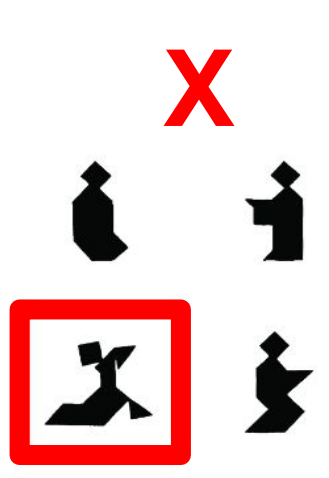
\includegraphics[height=4em]{images/limited-wrong.png} 
\phantom{m} 
\includegraphics[scale=.1]{images/limited-correct.png}};
	\node[align=center, anchor=center] at (10,-6) {Group \\ coherence: \\ Feedback};
	\node[illus, anchor=west] () at (11.2,-6) {Full feedback \\  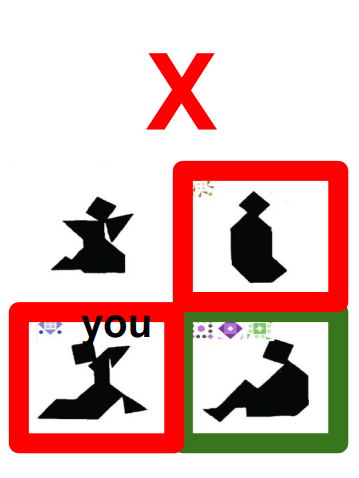
\includegraphics[height=4em]{images/full-wrong.png}  \phantom{m} 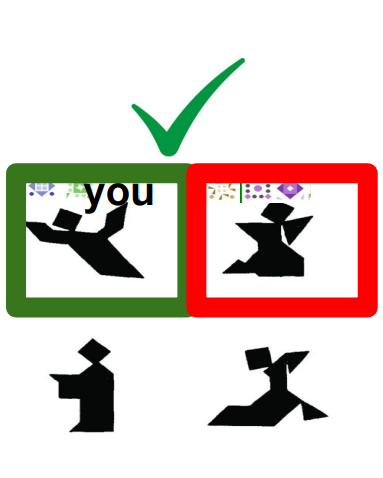
\includegraphics[scale=.1]{images/full-correct.png}	};

		
		\node[illus, anchor=north west] () at (8.75, 3.5) {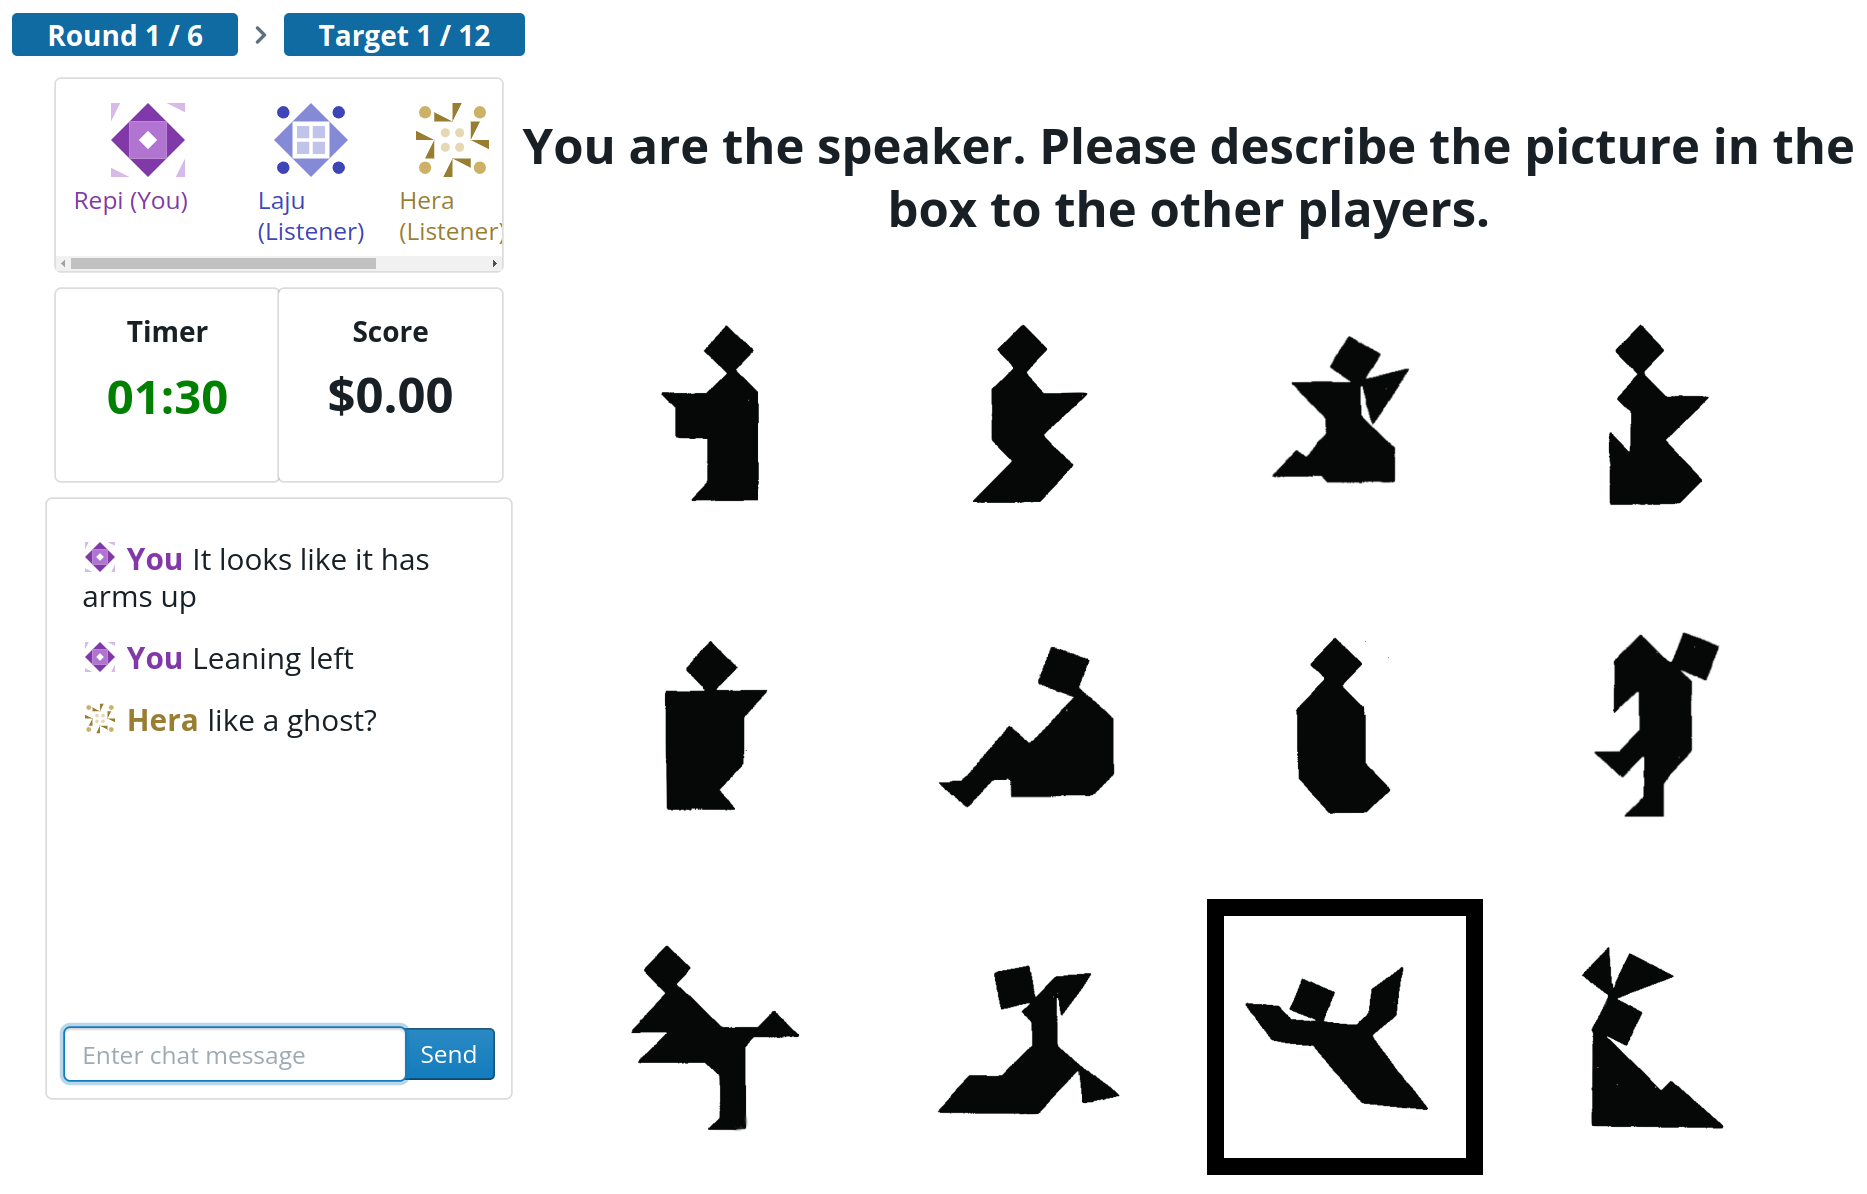
\includegraphics[width=15em]{images/diagram.png}};
		\node[anchor=north west] () at (11, 4) {Trial};
		
		\node[illus, anchor=north west, minimum width=18.5em, minimum height=14.5em] (block) at (8.5, 4) {};
		\node[anchor=north west] () at (11, 4.5) {Block};
		\node[anchor=north west] () at (12.5, -.5) {x 12 images};
		\node[anchor=north west] () at (12.5, -1.1) {x 6 iterations};
		

		
		
		
	\end{tikzpicture}
	




	

\end{document}